Les transcriptions manuelles sont faites à partir des fichiers wav et celles de MuseScore à partir des fichiers MIDI.\\
\section{Partitions entières}
Mettre ici des partitions entièrement transcrites.
\section{Comparaisons de transcriptions}
\subsection*{0. Prise en main}
Pour la prise en main, les transcriptions manuelles ont été faites avec musescore au lieu de lilypond.
\textbf{Premiers tests sur drummer\_01/session3}\\

\textbf{\textit{Exemple 1 : 10\_rock-folk\_90\_beat\_4-4}}\\\\
\textbf{manuelle}\\
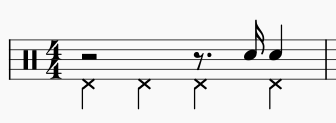
\includegraphics[height=25mm, width=70mm]{images/transcriptions_manuelles/0_prise_en_main/0_tests_drummer_01__session3/manuel_0.png} \\
\textbf{musescore}\\
\includegraphics[height=25mm, width=70mm]{images/transcriptions_manuelles/0_prise_en_main/0_tests_drummer_01__session3/musescore_0.png} \\
\begin{itemize}
	\item Erreur d’indication de mesure ;
	\item Mauvaise transcription d’une noire.\\
\end{itemize}
La noire du 4ème temps se retrouve sur le premier temps de la mesure suivante et elle se transforme en un triolet de double croches dont seules les deux premières seraient jouées.\\\\
\textbf{\textit{Exemple 2 : 10\_rock-folk\_90\_beat\_4-4}}\\\\
\textbf{manuelle}\\
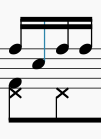
\includegraphics[height=30mm, width=25mm]{images/transcriptions_manuelles/0_prise_en_main/0_tests_drummer_01__session3/manuel_1.png} \\
\textbf{musescore}\\
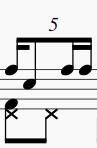
\includegraphics[height=30mm, width=25mm]{images/transcriptions_manuelles/0_prise_en_main/0_tests_drummer_01__session3/musescore_1.png} \\
\begin{itemize}
	\item Erreur de quantification : les doubles croches ont été interprétées en quintolet;\\
\end{itemize}
\textbf{\textit{Exemple 3 : 2\_jazz-swing\_185\_beat\_4-4}}
\\\\
\textbf{manuelle}\\
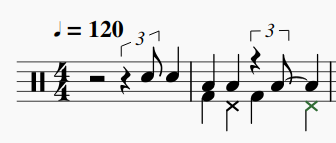
\includegraphics[height=30mm, width=65mm]{images/transcriptions_manuelles/0_prise_en_main/0_tests_drummer_01__session3/manuel_2.png} \\
\textbf{musescore}\\
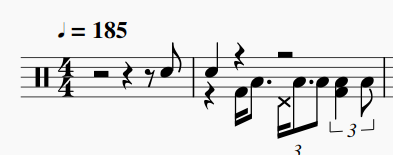
\includegraphics[height=30mm, width=65mm]{images/transcriptions_manuelles/0_prise_en_main/0_tests_drummer_01__session3/musescore_2.png} \\
\begin{itemize}
	\item L’indication de mesure est correcte mais tout a été décalé d’un temps car la première noire sur la caisse claire est jouée sur le 4ème temps et non sur le premier temps de la deuxième mesure comme l’indique la transcription de musescore.
	\item Les toms basses des 1er et 2ème temps de la mesure musescore auraient dû être sur les temps et non décalés d’une double croche vers la droite.\\
\end{itemize}
\textbf{Solutions aux pb rencontrés}\\\\
Existe-t-il un moyen de rectifier les erreurs d’indication de mesure et de décalage de temps des partitions MuseScores.\\
\begin{itemize}
	\item Changer dans manuellement dans MuseScore l’indication de mesure\footnote{\url{https://musescore.org/fr/manuel/indications-de-mesure}} fonctionne avec la transcription du MIDI. \\\\ 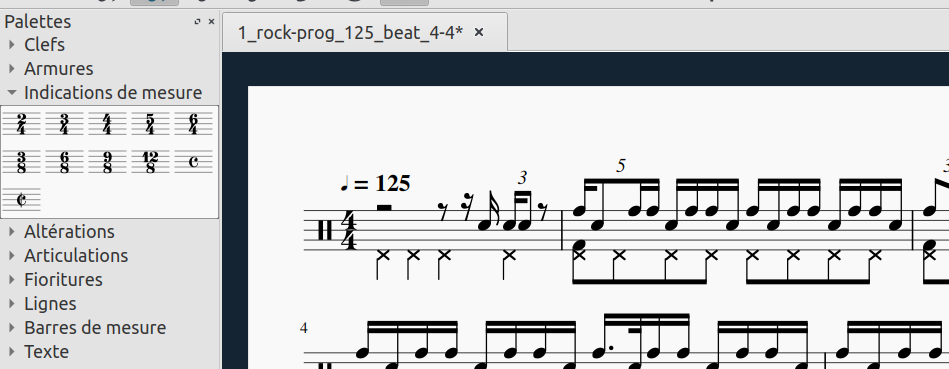
\includegraphics[height=30mm, width=65mm]{images/transcriptions_manuelles/0_prise_en_main/0_tests_drummer_01__session3/solution_0.png} \\
	\item Pour décaler tout d’un temps, on peut sélectionner les mesures en question en cliquant sur la première note de la séquence et en maj-cliquant sur la dernière, puis Ctrl-X Ctrl-V pour replacer le tout au bon endroit.\footnote{\url{https://musescore.org/fr/node/276292}}\\
\end{itemize}

\textit{À partir de la prochaine section, les indications de mesures erronées ou les décalages de temps qui ont des répercussions sur l’ensemble de la partition seront corrigés avant l’analyse.}\\\\
\textbf{Seconds tests sur drummer\_01/session1}\\\\
\textbf{\textit{Exemple 1 : 1\_funk\_80\_beat\_4-4}}
\textbf{manuelle}\\
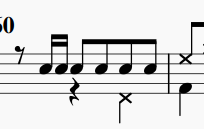
\includegraphics[height=25mm, width=40mm]{images/transcriptions_manuelles/0_prise_en_main/1_drummer_01__session1/Manuelle_0.png} \\
\textbf{musescore}\\
\includegraphics[height=25mm, width=40mm]{images/transcriptions_manuelles/0_prise_en_main/1_drummer_01__session1/musescore_0.png} \\
\begin{itemize}
	\item On dirait que lorsque certaines notes sont proches, elles se resserrent et suppriment celles qui aurait dû être sur le temps.\\
\end{itemize}
\textbf{\textit{Exemple 2 : 1\_funk\_80\_beat\_4-4}}
1\_funk\_80\_beat\_4-4\\\\
\textbf{manuelle}\\
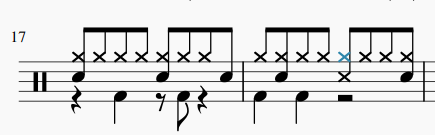
\includegraphics[height=25mm, width=70mm]{images/transcriptions_manuelles/0_prise_en_main/1_drummer_01__session1/Manuelle_1.png} \\
\textbf{musescore}\\
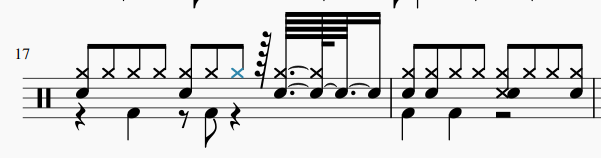
\includegraphics[height=25mm, width=70mm]{images/transcriptions_manuelles/0_prise_en_main/1_drummer_01__session1/MuseScore_1.png} \\
\begin{itemize}
	\item La caisse claire de la 2ème croche du 4ème temps de la 1ère mesure se transforme en une combinaison de quadruple/quintuple/double croches liées qui commence par un soupir et finit en débordant sur le premier temps de la mesure suivante. 
\end{itemize}
\newpage
\subsection*{1. Transcription des flas}
À partir de maintenant, les transcriptions manuelles seront faites avec LilyPond.
\subsubsection{Sur la question des flas}
Des exemples de notation flas tom/caisse-claire existent dans des partitions récentes (rythmique binaire J.-F. Juskowiak).\\
$\Rightarrow$ Ils faudra donc les prendre en compte dans les comparaisons de transcriptions.
De gauche à droite : transcription musescore, transcription manuelle.\\
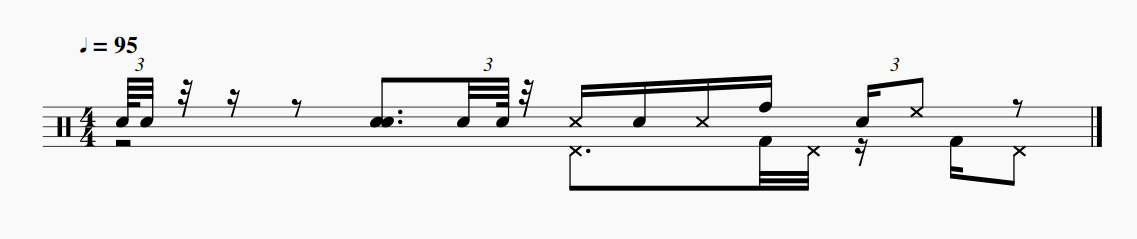
\includegraphics[height=20mm, width=80mm]{images/transcriptions_manuelles/1_transcriptions_flas/124_funk_95_fill_4-4_0.png}
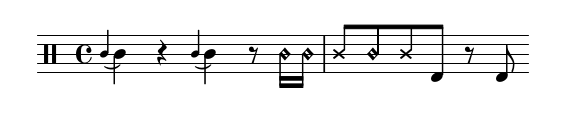
\includegraphics[height=20mm, width=80mm]{images/transcriptions_manuelles/1_transcriptions_flas/124_funk_95_fill_4-4_1.png}\\
Il manque des charley, je dois trouver comment faire des accords avec des têtes de notes différentes.\\\\
\subsection*{2. Autres}
- Chercher des exemples de silences, tuplets.\\
- Faire les observations avec des notations plus ou moins chargées.